% !TEX root = pfe-book3.tex
%!TEX TS-program = pdflatex
%!TEX encoding = UTF-8 Unicode


\cleardoublepage
%\mainmatter
\chapter{Electrical Structure of Matter}
\label{ch-02}

\section{Minimum Quantity of Electricity}
For many years, all the information on electrical phenomena known to physicists consisted in the certainty that electricity was something like a liquid. The following joke was still enjoying success at the turn of the century. Wishing to make a laughing-stock of a poorly prepared student, the examiner says, ``Well, since you can't answer all my other questions, try this simplest one: What is electricity?''

The student answers, ``On my word of honour, I knew, Professor Jones, but I have forgotten.''

At this the examiner exclaims, ``What a loss for mankind! There was only one person in the whole world who knew what electricity is, and he has forgotten!''

The first hints that electricity consists of special particles instead of being a continuous fluid, and the certainty that these electrical particles are related in some way to atoms were obtained in studying electrolysis.

In conducting experiments on the dissociation of substances dissolved in water when a current is passed through the solution, the English scientist Michael Faraday (1791-1867) found that the same electric current deposits various amounts of substances on the electrodes depending on what chemical compound is dissolved in the water. Faraday discovered that 96 500 coulombs pass through the electrolyte to deposit one gram-atom of a monovalent substance, and that twice as much is required to deposit one gram-atom of a bivalent substance.

Maybe you think that when Faraday obtained these results he cried, ``Eureka!'' and announced that he had discovered the essential character of electricity? Not at all. The gifted experimenter permitted himself no such illusions. Faraday, in any case, with respect to electric current, behaved like our mythical investigator of the preceding chapter. He considered it feasible to make use of only those concepts that can be characterized by numerical values.

``How so?'' the reader may ask. It has been shown that \num{6.023d23} atoms (you recall that this is Avogadro's number) carryover 96 500 coulombs of electricity. Consequently, if we divide the second figure by the first, we obtain the quantity of electricity carried by any monovalent atom. The quotient is \num{1.6d-19} coulombs. This then is the minimum quantity of electricity, or the ``atom of electricity'', or the ``elementary charge''.

But Avogadro's number was not determined until 1870. It was only then (just think of it; a mere hundred years ago) that physicists who like to devise hypotheses (their frame of mind and mentality greatly differentiate them from the investigator who tries to keep within the bounds of the phenomenon being studied) decided that the following assumption is highly probable. Along with electrically neutral atoms, particles exist that carry one or several elementary charges of electricity (positive or negative). Atoms carrying a positive charge (\emph{cations}) are deposited on the cathode during electrolysis; those carrying a negative charge (\emph{anions}) are deposited on the anode.

Molecules of salts dissolved in water are dissociated into anions and cations. A molecule of common salt, sodium chloride, for instance, dissociates into a positive ion of sodium and a negative ion of chlorine, rather than into an atom of sodium and an atom of chlorine.
 
\section{Ion Flow}
Naturally, electrolysis only suggests to the investigator the idea that electrical particles exist.

Many procedures were proposed at the turn of the last century for converting molecules into charged fragments (a phenomenon called ionization). Methods were found for producing directed streams of charged particles and, finally, procedures were worked out for measuring the charge and mass of ions. Physicists gained their first knowledge of ion flow when they connected a glass tube with rarified gas into a d-c circuit. At a low voltage across the electrodes sealed into the glass of the tube, no current is observed. But it turned out to be quite simple to convert the rarified gas into a conductor. The gas can he ionized by the effects of $X$-rays, ultraviolet light or radioactive radiation. We can even manage without such special measures if we apply a higher voltage to the tube terminals.

Gas thus becomes a conductor of electric current. We can assume that the molecules are broken up into anions and cations. The anions travel toward the positive electrode and the cations toward the negative one. An important breakthrough in investigating this phenomenon was the production of a stream of particles. This is done by making a hole in one electrode and accelerating the ions of a single sign passing through the hole with an electric field. By means of a diaphragm, we can obtain a narrow beam of anions or cations travelling at considerable velocity. If such a beam is directed to a screen of the type on a TV picture tube, we see a bright spot. By passing the ion beam through two mutually perpendicular electric fields and varying the voltage over the capacitors setting up these fields, we can make the spot wander over the screen.

Using a similar device, we can determine one of its most important parameters: its charge-to-mass ratio.

In an accelerating field, ions gain energy equal to the work done by the electric forces, i.e.
\begin{equation*}%
\frac{mv^{2}}{2} =eV
\end{equation*}
We know the applied voltage, and the velocity of the particles can be measured by various essentially differing ways. We can, for instance, measure the deviation of the spot of light on the screen. It is clear that the longer the path of the particle and the lower its initial velocity, the greater the deviation. This problem can be quite rigorously solved. It resembles the calculation of the path of a stone thrown horizontally.

There are also methods for direct measurement of the time it takes the ion to travel over its whole path.

Hence, we know the voltage and the ion velocity. What can we calculate from the results of this experiment? It follows from the equation that we can find the ratio of the charge of the particle to its mass. It is a pity, however, that we cannot separate the charge from the mass no matter how we change the conditions of the experiment, or what deviations and accelerations of the particles we use. Only on the basis of data obtained by chemists, and the value of the elementary charge obtained in electrolysis, can we come to the reliable conclusion: the charges of all monovalent ions are the same, the charges of bivalent ions are twice as much, those of trivalent ions are three times as much, etc. The differences in the charge-to-mass ratios, which can be measured with exceptional precision, indicate a method for measuring the mass of the ion.

This is why the instrument, of exceptional significance in chemistry and chemical technology and based on the principle of the simple experiment described above, is called the mass spectrograph (see Book~4), though, in fact, it measures the charge-to-mass ratio of ions.

\section{Electron Beam}

We shall not trace the zigzag course of historical events that led physicists to the unshaken conviction that a minimum portion of electricity not only exists, but has a material carrier, which they called the electron. Instead we shall describe an experiment that is demonstrated in school lessons in physics.

The apparatus used in this experiment was once called a cathode, or cathode-ray, tube. Now it is called an electron-beam tube or an electron gun or an oscillograph. If your school days are far behind and you had no opportunity to become acquainted with this instrument, no matter, you have seen and see plenty of them now: an electron-beam tube is the main component of your television set. On the somewhat flattened end, or screen, of the tube, the electron beam draws the moving pictures that we sometimes view with pleasure and which always enable us to kill time.
\begin{figure}[!ht]
\centering
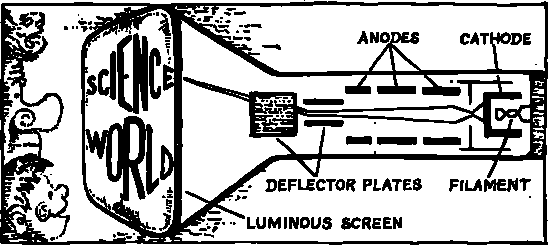
\includegraphics[width=\textwidth]{figures/fig-02-01.pdf}
\caption{A cathode-ray tube or electron beam tube.}
\label{fig-2.1}
\end{figure}

Let us return, however, to the school experiment. A diagram of such a tube is illustrated in \figr{fig-2.1}. The tube is ideally evacuated; all molecules th.at could dissociate have been pumped out. However, after a current (called the cathode current) heats the filament to incandescence, the filament heats the cathode. Then, when the cathode and anode are connected to the corresponding terminals of the voltage source, you can observe a bright spot on the fluorescent screen. You can now establish by means of a measuring instrument that an electric current passes from the anode to the cathode. It is quite naturally called the anode current.

Since the current passes through a vacuum, you must come to the conclusion that the incandescent cathode emits negatively charged particles. This is called \emph{thermoelectron}, or \emph{thermionic emission}. Any incandescent body has this property.

These particles (we shall not hide from the reader that they are electrons) travel toward the anodes, which are designed as cylinders closed at one end and with a tiny round hole in the centre of the bottom. The electrons are emitted as a narrow beam, which can be investigated in the same way as described above for a beam of ions.

Convinced by the spot on the luminous screen that the cathode is emitting electrons, we proceed to find their charge-to-mass ratio by means of deflector plates. The results are the following. This ratio for the electron is 1840 times greater than for the lightest ion, namely, the hydrogen ion. This leads us to tho conclusion that the hydrogen ion is 1840 times heavier than an electron. Consequently, the mass of the electron is \SI{9d-28}{\gram}. 

Here our reader may rightly object, saying that we are in too much of a hurry. On the face of it, you cannot come to the conclusion that the mass of an electron is less than that of an ion only by measuring their charge-to-mass ratio. Maybe the charge of the positively charged ion and that of the electron are entirely different?

The charge-to-mass ratio of the electron was determined way back at the end of last century by the brilliant English physicist Sir Joseph John Thomson (1856-1940). His friends called him J. J. (This abbreviation, so often found in memoirs and biographies, is due less to the fact that the English like abbreviations so much as to the fact that another famous British physicist of the same name lived and worked during the 19th century. He was William Thomson (1824-1907). A peerage was bestowed upon him for his scientific merits and he became Lord Kelvin.) The cathode tube used by J. J. Thomson was, of course, not as highly perfected as an up-to-date oscillograph. Thomson was perfectly aware that his measurements only showed that the discreteness of electric charge was quite feasible and that a minimum portion of electricity could exist.

Strange as it may seem, even though many physicists had observed the behaviour of cathode and anode beams, there were still many supporters of the hypothesis that these beams were of a wave nature. These investigators found no necessity for admitting that the currents passing through a metal conductor, through a liquid, and through a gas or vacuum are near of kin. They insisted on more direct proofs. We can, of course, understand their point of view: circumstantial evidence is insufficient to convert a hypothesis into a fact.

Hence, it was essential, first of all, to substantiate the validity of the hypothesis by direct measurements of the size of the electric charge of particles. These measurements, far from unsuccessful, were begun by Thomson and his colleagues in the early years of the 20th century. The most precise measurements were made in 1909 by the American physicist Robert Andrews Millikan (1868-1953).


\section{Millikan's Experiment}
The idea of the discreteness of electricity seems quite bold, and the determination of the elementary charge, with an account of which we began this chapter, can be treated in a different way. What is wrong with contending that anions actually exist and that negative electricity is a liquid entrained by the positive ion? One ion picks up one amount of this liquid, another ion picks up another amount, and the experiment indicates some average value. This is a reasonable explanation, is it not?

As mentioned above, Thomsons experiments were a powerful, but not decisive, argument in favour of the existence of the electron. No need then to prove the vital importance to physics of an experiment that could demonstrate the existence of the elementary charge of electricity so obviously that all doubts were instantly discarded. Such an experiment was devised in 1909 by Robert Millikan. I shall not mention here the other works of this famed scientist, but this single investigation was sufficient to put his name in all physics textbooks.
	
The principle of this ingenious experiment is based on a simple fact. Just as a glass rod rubbed by a piece of fur acquires electrical properties, other substances behave in a similar way. This is called electrification by friction. But, strictly speaking, what reason have we to think that this property is inherent in only solid bodies? If we spray tiny droplets of oil into a chamber, will they become electrified by the friction as they pass the orifice of an atomizer? We find that they will. This can be demonstrated by what is, in principle, quite simple apparatus. We spray a stream of fine oil droplets into the space between two horizontal capacitor plates enclosed in a chamber. Then we arrange a suitable microscope to enable us to observe the droplets. Until an electric field is set up, the droplets naturally fall downward by gravity. The droplets are very light and the force of gravity is almost immediately counterbalanced by the air resistance so that they drift downward at uniform velocity. As soon as we apply a voltage across the plates, we observe a definite change in the behaviour of the droplets. Their motion is either accelerated or decelerated, depending upon the direction of the electric field. Millikan chose the direction that slowed down the droplets. By gradually increasing the intensity of the field, he could, so to speak, hold the droplet at rest between the plates. For hours, he observed a single oil droplet. Varying the field, he could control its motion or stop it at will.

What can we calculate by means of this experiment? First we shall discuss the data obtained in observation before setting up the electric field. The equality of the force of gravity and the air resistance can be expressed by the equation
\begin{equation*}%
mg=av
\end{equation*}
The density of the oil can be determined by an independent experiment; the diameter of the droplet is measured by the microscope. After this the mass of the droplet is readily calculated. The droplet drifts slowly downward and by engraving scale divisions on the microscope lens we can measure the velocity $v$ of the droplet with a stopwatch with a sufficient degree of accuracy. Then, substituting these quantities into the preceding equation, we obtain the resistance coefficient $a$.

Next we switch on the field. It proves most convenient to select a field intensity for which the droplet begins to rise at uniform velocity. We have thus added a third force to the two previous ones; it is the force exerted by an electric field whose intensity $E$ is known (the ratio of the voltage across the plates to the distance between them). Upward motion at uniform velocity means that the three forces counterbalance one another. The condition for such equilibrium is given by
\begin{equation*}%
qE - mg = av'
\end{equation*}
The new value $v'$ of the velocity can be measured with the same microscope and stopwatch. All the quantities in the equation are known now except the charge of the droplet. We next calculate the charge and enter the value in a journal for experimental data of the kind kept by all scrupulous experimenters.

Now we have come to the main idea of the oil-drop experiment. The current in an electrolyte, reasoned Millikan, is carried by ions of different signs. But ions can be formed in a gas as well. Air can be ionized by various procedures. We can, for instance, place out whole arrangement near an $X$-ray tube. Then the $X$-rays ionize the air. This was well known in 1909. But if a droplet is charged it attracts ions of the opposite sign. As soon as all ion becomes attached to a droplet, the charge of the latter is changed, and, with its charge, its velocity is also changed. This new velocity is immediately determined by another measurement.

Observations proved the correctness of the idea. When the $X$-ray tube was switched on, every now and then various droplets would abruptly change their velocity, keeping his eye on a single droplet, the observer measured the difference in velocities before and after the $X$-rays were switched on. From the formula given above, the value of $q$ was readily found.

Have you not guessed yet what all this is being done for? Think again. If there is such a thing as an elementary electric charge, then the measured value should equal it if a single monovalent ion joins the droplet or be a multiple of the elementary charge if several ions become attached to the droplet.


Conducting his experiment with droplets of oil, water, mercury and glycerine, and reversing the charge of the droplets, Millikan filled his data journal with hundreds of values of $q$, and they all were equal to or a multiple of a single value, the same that had been found by the investigators of electrolysis.

When Millikan published his results, even his most skeptical opponents were convinced that the electric charge is found in nature in discrete portions. Strictly speaking; however, Millikan's experiments do not directly prove the existence of the electron as a particle.

But hypotheses foreshadow facts. Some scientists were sure that electricity is of a granular nature as far back as the beginning of the 19th century. The charge of the ion was first calculated in 1881 by the Irish physicist George Johnstone Stoney (1826-1911) and ten years later he first proposed the term \emph{electron}, not for the particle, but for the charge of a monovalent negative ion. J.J. Thomson's experiments compelled the great majority of physicists to believe in the existence of the electron as a particle. The German physicist Paul Karl Ludwig Drude (1863-1906) was the first to unambiguously define the electron as a particle carrying an elementary charge of negative electricity.

Thus the electron had been generally recognized before it was ``seen''.

Direct proof of the existence of electrons was obtained later by precise experiments. A weak beam of these particles was directed onto a screen where they can be counted one by one. Each electron causes a flash on a luminescent screen. Luminescent screens have long been replaced for this purpose by special counters named after their inventor, the German physicist Hans Wilhelm Geiger (1882-1945). In a word, the idea of such a counter is that a single electron, like the trigger of a revolver, initiates a strong current pulse, which can be readily registered. This enables the physicist to establish the number of electrons entering a trap per second. If this trap is a metallic bulb into which the electrons fly, the bulb is gradually charged with a quantity of electricity large enough to be precisely measured. To find the charge of the electron it is sufficient to divide the quantity of electricity by the number of captured electrons.

Only after this can we contend that the existence of the electron is no longer a hypothesis; it is a fact.

We have reviewed at racing-car speed the discoveries that laid the foundations of modern physics. Such, however, is their fate. New matters crowd out the old, and even cardinal events, occurring during the construction of the cathedral of Science, become only material for historians.

Now, perhaps, we can answer the question: What is electricity? An electric fluid is a current of electrical particles. A body is electrically charged when the number of particles of one sign exceeds that of the other sign.

``Well, what a feeble explanation,'' retorts our indignant reader. ``And what then is an electrical particle?''

``Isn't it perfectly clear? A particle is said to be electrical if it interacts according to Coulomb's law.''

``And is that all?'' asks the puzzled reader.

``All that concerns the answer to your question,'' answers the physicist. ``But ahead of us are answers to many other interesting questions. We have not yet mentioned the cases in which we shall find elementary particles of positive electricity. We shall also find out that electrical particles are characterized by other properties besides their charge and mass.''

First, however, we shall discuss the structure of the atom.

\section{Model of the Atom}
How is an atom built up of electrical particles? The answer was obtained by means of rays emitted by radium. We shall discuss this wonderful substance and the extensive family of natural and artificial radioactive elements in Book~4 of this series. For the time being it is sufficient for us to know that radium constantly emits penetrating electromagnetic radiation (gamma rays), a stream of electrons (formerly called beta rays) and alpha rays, which consist of doubly charged ions of helium atoms.

In 1911, the eminent New Zealand-born physicist Sir Ernest Rutherford (1871-1937) proposed the so-called planetary model of the atom, based on his careful investigations of the scattering of alpha particles by various substances. Rutherford conducted his experiments with thin gold leaf, only a tenth of a micron in thickness. He found that out of 10 000 alpha particles only one was deflected through an angle exceeding \ang{10}.

In these strikingly simple experiments, the passage of each separate particle was recorded. Up-to-date techniques, of course, enable such measurements to be made entirely automatically.

It becomes clear then that the atom consists mainly of empty space! The rare head-on collisions should be interpreted as follows: inside the atom there must be a positively charged nucleus, This nucleus is surrounded by electrons. They are extremely light and therefore present no appreciable obstacles to the alpha particles. The electrons slow down the alpha particles, but a collision with each separate electron cannot deflect the particle from its path.

Rutherford assumed that the forces of interaction between the atomic nucleus and alpha particle, which are of like charge, are Coulomb forces. Assuming further that the mass of the atom is concentrated in its nucleus, he calculated the probability of the particle being deflected through the given angle and obtained splendid coincidence of theory with experimental data.

That is how physicists check the models they have devised.

``So the model predicts the experimental results?'' 

``Yes.''

``Which means that it represents reality?''

``Why so categorical? A model explains a series of phenomena and so is a good one. Its refinement is a matter for the future.''

The results of Rutherford's experiments swept aside all doubts as to the validity of the following statement: electrons are subject to Coulomb forces and travel about the nucleus.

The theory also led to certain quantitative estimates which were later confirmed. The size of the very smallest atomic nuclei turned out to be about \SI{d-13}{\centi\meter} while the size of the whole atom is of the order of \SI{d-8}{\centi\meter}.

Comparing the experimental results with the calculations, physicists were able to estimate the charges of colliding nuclei. These estimates played a vital, if not the main, role in interpreting the periodic law of the structure of the elements.

Thus, we have built the model of the atom. But the following question is immediately posed: Why don't the electrons (negatively charged particles) fall into the nucleus (positively charged)? Why is the atom stable?

``There is nothing strange about this,'' reasons the reader. ``The planets do not fall on the sun. A force of electrical origin, like the gravitational force, is centripetal and provides for circular motion of the electrons about the nucleus.''

But the point is that the analogy between the planetary system and an atom is only superficial. As we shall find out further on, an atom must emit, from the point of view of the general laws of electromagnetic fields, electromagnetic radiation. But this is something we can ascertain without a knowledge of the theory of electromagnetism. Matter, i.e. atoms, is capable of radiating light and heat. Since this is so, the atom loses energy and the electron must finally fall into the nucleus.

What is the way out of this dilemma? It is quite simple. We must reconcile ourselves to the facts and elevate them to the rank of a law of nature. This step was taken in 1913 by one of the greatest physicists of our century, Niels Henrik David Bohr (1885-1962).

\section{Quantizing Energy}

Like all first steps, this step was relatively timid. We shall now present the new law of nature that not only saved Rutherford's atom, but forced us to the conclusion that the mechanics of large bodies is inapplicable to particles of small mass.

Nature is arranged so that a number of mechanical quantities, such, for instance, as angular momentum or energy, cannot have a continuous series of values for any system of interacting particles. On the contrary, the atom, now being discussed, or the atomic nucleus, to be discussed later, has its own sequence of energy levels inherent in only the given system. There is the lowest level (ground state). The energy of the system cannot be less than this value. In the case of the atom this means that there is a state in which the electron is at a certain minimum distance from the nucleus.

Changes in the energy of an atom can occur only in jumps. If the jump is ``upward''; it means that the atom absorbed energy; if it is ``downward'', the atom radiated energy.

We shall see further on how nicely, on this basis, the radiation spectra of various systems can be deciphered. 

The formulated law is called the \emph{law of the quantization of energy}. We can also say that energy is of a quantum nature.

It should be noted that the law of quantizing is of an entirely general nature. It is applicable not only to the atom but to any item consisting of thousands of millions of atoms. When we deal with large bodies, however, we may not ``notice'' the quantizing of energy. The point is that for an item consisting of a million million million atoms the number of energy levels are increased, roughly speaking, by a million million million times. These energy levels are so close to one another that they practically merge into a single band. Consequently, we cannot observe the discreteness of the energy values. Thus, the mechanics we discussed in Book~1 remains practically unchanged when we deal with large bodies.

In Book~2 we found that energy can be transferred from one body to another in the forms of work and heat. Now we are in a position to explain the difference between these two forms of energy transfer. The mechanical action (for example, in compression), the energy levels of the system are displaced. This displacement is very slight and can be detected only by precise experiments if the pressure is high enough. As to heat action, it consists in converting a system with a lower energy level to a higher one (in heating) or one with a higher energy level to a lower one (in cooling).

The quantizing of energy, like that of other mechanical properties, is a general law of nature. A great variety of consequences that follow strictly from this law can be confirmed experimentally.

Maybe you wonder why energy is quantized? There is no answer. Nature just happens to be made that way! Any explanation is a reduction of a particular fact to a more general one. We know today of no statement sufficiently general for the quantizing of energy to follow from it as a consequence. This does not imply, of course, that at some future date, in principle at least, sufficiently broad and comprehensive laws will be discovered for the principles of quantum mechanics to be their corollaries. However that may be, the law of quantizing is today one of the few great laws of nature that require no logical substantiation. Energy is quantized because -- it is quantized.

This law was established in such a general form during the years 1925-1927 in the works of the French physicist Louis Victor Pierre Raymond, Prince de Broglie (1892-1987) and the Austrian and German physicists Erwin Schr\"odinger (1887-1961) and Werner Karl Heisenberg (1901-1976). The branch of physics based on the quantizing principle (I forgot to mention that the word quantum means a specified quantity or portion) was named \emph{quantum}, or \emph{wave mechanics}. But why wave? This will be explained later on.

\section{Mendeleev's Periodic Law}

In 1869, the famed Russian chemist Dmitri Ivanovich Mendeleev (1834-1907) published the periodic law he discovered in the order of the chemical elements. We shall not give Mendeleev's periodic table here; it can be found in any school chemistry textbook. We need recall here only that when he arranged the elements in the order of their atomic weights Mendeleev noted that their chemical properties and certain physical features vary periodically in accordance with their atomic weight. 

In the table devised by Mendeleev, each element belongs to one of nine groups and to one of seven periods. He arranged the elements of the groups in columns so that the elements whose symbols are arranged one below the other possess the same chemical properties. He found that this could be done only if he assumed that certain as yet undiscovered elements existed. He left empty spaces (gaps) for them in his table. The exceptional foresight of this great scientist also led him to put the nickel atom in its ``proper'' place following cobalt, not withstanding the fact that the atomic weight of cobalt is somewhat higher.

Some of the gaps were filled during Mendeleev's life. This brought him world renown because it became clear that the compilation of this table was the discovery of a great law of nature rather than a mere formality.

The essence of the atomic number assigned by the table to each chemical element became evident after the physicists had no more doubts about the validity of Rutherford's planetary model of the atom and of the quantizing of energy. What does this number mean? The answer turned out to be extremely simple. The number of an element in the periodic table, its atomic number, is equal to the number of electrons rotating about the nucleus. We can say that the atomic number of an element is the positive charge of its nucleus expressed in units of charge of its electrons.

Mendeleev's periodic law, the principle of energy quantization and a study of the characteristic optical and $X$-ray spectra of atoms (to be discussed further on) cleared up the reason for the same chemical behaviour of atoms in any one column of Mendeleev's table.

The energy of an atom is the energy of interaction between the electrons and the nucleus. Since energy is quantized, it is logical to assume that the electrons of each atom can be arranged in a series according to their energies. The first electron is most strongly bonded to the nucleus, the second, more weakly, and the third, still more weakly, etc. Thus the electrons of an atom are arranged in energy steps. We have not been misled by our logical reasoning, but investigations have more accurately defined this concept. In the first place, each energy step can be occupied by two rather than a single electron. True, these electrons are identical; they differ from each other in a property known as \emph{spin}. This is a vector quantity. Hence, people who prefer a more visual concept can imagine that a filled step has two ``tiny dots'' with arrows, one arrow pointing ``downward'' and the other ``upward''.

The word ``spin'' is of the following origin. One of its definitions is to rotate swiftly, like a top. To explain the difference between two electrons occupying the same step, one was to imagine one electron as rotating clockwise and the other counterclockwise about their axes. This model was suggested by the superficial resemblance between the atom and the planetary system. If an electron is something like a planet, then why not allow it to rotate about its axis? Again I must distress my readers: it is quite impossible to visualize the spin of an electron. But it can be measured, as we shall see in the next chapter. 

This, however, is not the only significant conclusion that we can reach (by a careful examination of atomic spectra). A second conclusion is that the energy steps can be at unequal distances from one another and can be divided into groups.

Following the first step, called the $K$-level, is an energy gap. This is followed by a group of eight electrons, denoted by the letter $L$, and then a group of 18 electrons, denoted by the letter $M$, etc. We shall not describe here the locations of the levels and the order in which they are filled for all atoms. It is not a simple picture and its description would require much space. Details play no appreciable role in our small book. I mentioned the energy steps only to explain the similarity of atoms located in a vertical column of Mendeleev's table. It was found that they have an equal number of electrons in the upper group of steps.

This clears up the chemical concept of the valency of an atom. Thus, lithium, sodium, potassium, rubidium, cesium and francium have a single electron in the upper group of steps. Beryllium, magnesium, calcium, etc. have two electrons in the upper group of steps. The valence electrons are the most weakly bonded in the atom. Therefore, in ionizing atoms of the first column, singly charged particles are most easily formed. Ions of beryllium, magnesium and others usually carry two charges, etc.

\section{Electrical Structure of Molecules}

Chemists call the molecule the tiniest representative of a substance. Most physicists use this word only when this tiniest representative really exists as a separate small body.

Do molecules of common salt exist? ``Of course!'' answers a chemist and writes the formula \ce{NaCl}. Common salt is sodium chloride. A molecule consists of one atom of sodium and one of chlorine. This answer, however, is only formally valid. Actually, we cannot find pairs of these atoms behaving as a single whole neither in crystals of common salt, nor in a solution of salt in water, nor in the vapour of sodium chloride. As we mentioned in Book~2, each atom of sodium in a crystal is surrounded by six chlorine neighbours. All of these neighbours possess equal rights and there is no way to find which one ``belongs'' to the sodium atom.

Let us dissolve common salt in water. We find that the solution is an excellent conductor of electric current. Rigorous experiments, discussed above, can be conducted to demonstrate that the electric current is a stream of negatively charged atoms of chlorine travelling in one direction and a stream of positively charged atoms of sodium travelling in the opposite direction. Hence, in a solution, atoms of chlorine and sodium do not form strongly bonded pairs of atoms.

After we have established the model of the atom, it becomes clear that an anion of chlorine is an atom of chlorine with an ``extra'' electron. A cation of sodium, on the contrary, has a ``shortage'' of one electron.

Can this lead us to the conclusion that a solid body is also built up of ions rather than atoms? Yes, it can. This can be proved by many experiments on whose description we shall not dwell here.

What about the vapour of sodium chloride? Here again we find no molecules. The vapour of sodium chloride consists of ions or of various extremely unstable groups of ions. We can speak of the molecules of ionic compounds only in the chemical meaning of the word.

Ionic compounds all dissolve in water. Such solutions, classical examples being simple metal salts, such as sodium chloride, have good conductivity and are therefore called strong electrolytes.

We can give several examples of substances built up of genuine molecules, molecules in the physical meaning of the word. They are oxygen, nitrogen, carbon dioxide, hydrocarbons, carbohydrates, steroids, vitamins, etc. This list could be continued to great length.

All classifications are always somewhat arbitrary. Therefore, I must warn the reader that sometimes we find cases in which the substance consists of physical molecules when it is in one state of aggregation, but does not when it is in other states. These substances include such vital ones as water. Water vapour molecules are undoubtedly separate bodies. But it is a difficult matter to ``outline'' a single molecule in ice crystals and to contend that these atoms of hydrogen are bonded only to this particular atom of oxygen.


Be that as it may, the class of molecular crystals is vastly extensive.

In Book~2 we have already discussed the structure of molecular crystals. Recall that in a crystal of carbon dioxide (\ce{CO2}) the carbon atom has two very close oxygen neighbours. In all other cases, in investigating the structure of a molecular crystal, we can readily see that it is possible to break down the crystal into intimately arranged groups of atoms.

If they are so closely located, they must be bonded by high forces. This is true. The forces bonding atoms belonging to a single molecule are, roughly speaking, a hundred or even a thousand times greater than the forces acting between atoms of neighbouring molecules.

Just what is this intramolecular bond? It is sufficiently clear that we shall not be able to manage by using only concepts of the mutual attraction of electrically charged negative and positive ions. We know that the molecules of oxygen, nitrogen and hydrogen consist of identical atoms. It is impossible to assume that one atom loses and the other atom gains an electron. Why on earth should an electron prefer to stay near either one of two identical atoms?

The principle of the intramolecular bond was grasped only with the evolution of quantum mechanics. We have just mentioned that the energy of any system is quantized and that two electrons of opposite spin can occupy a single energy level. In addition, an interesting consequence follows from one of the basic hypotheses of quantum mechanics. It was found (and this is no hypothesis, but a strict mathematical derivation which we do not give because of its complexity) that the lowest energy value assumed by an electron depends upon the size of the region within which it travels. The greater the size, the lower the energy of this ``zero level''.

Now imagine that two atoms of hydrogen approach each other. If they merge into a single system, the ``apartment'' for each electron is approximately doubled. Two
electrons with opposite spin can peacefully coexist in a single ``apartment''. Consequently, such life together is expedient. The region in which the electrons exist has appreciably increased. This means that the total energy of the system has decreased after the two atoms merge together. By now we have completely mastered the fact that any system, if there are any such possibilities, tends to go over to the state with minimum energy. For the same reason, a ball, left to itself, rolls downhill.

Thus, the formation of a chemical bond implies the collectivization of the electrons. There is a certain number of electrons (said to be inner-shell electrons) that rotate about the nuclei of the atoms, but some (outer-shell) electrons include at least a pair of nearest atoms in their motion or even may travel among all the atoms of the molecule.

We can recognize a substance built of molecules by its electrical properties. A solution of such a substance conducts no current. The molecules do not break down into parts and a whole molecule is electrically neutral. In liquids and vapours, the molecules retain their structure; the whole group of atoms travels as a single whole, with translatory or rotary motion. Atoms belonging to such molecules can only vibrate about their equilibrium positions.

A neutral molecule carries no electric charge. But do not hasten to the conclusion that such a molecule does not set up an electric field. If the molecule is asymmetric, the centres of gravity of its positive and negative charges almost certainly do not coincide. It is intuitively clear that the centres of gravity of the two charges coincide in such molecules as oxygen and nitrogen, consisting of two identical atoms. Nor is it difficult to understand that in a molecule of a gas such as carbon monoxide (\ce{CO}) these centres may be displaced with respect to each other. If there is such a displacement, the molecule is said to have a dipole moment.

This term has the following origin: a dipole molecule behaves like a system of two point charges (one point is the centre of gravity of the negative charges and the other is the same for the positive charges). A dipole is specified by the size of the charge and the dipole arm, i.e. the distance between the centres of gravity.

Do not require proof that an asymmetric molecule has an electric dipole moment. We can dispense with a theoretical discussion because the existence of a permanent (or, as they also say, rigid) dipole moment can be readily demonstrated by experiments.

\section{Dielectrics}

We can place equality signs between a dielectric, a nonconductor of current and an insulator.

\emph{Dielectrics} include molecular gases, molecular liquids and solutions of solids made up of molecules. Solid dielectrics include glass, both organic and nonorganic (silicate, borate, etc.); polymer substances, built up of giant molecules; plastics, molecular crystals, as well as ionic crystals.

We reminded the reader in \hlgray{Chapter}~\ref{ch-01} that the capacitance of a capacitor increases when we insert any dielectric into the space between the plates. Imagine that the capacitor was connected to a source of constant voltage. The capacitance increased even though the voltage remained the same. This means that an additional charge approached the capacitor plates. It would seem that the field intensity must also increase. It has not changed, however, because it is the quotient of the voltage divided by the distance between the plates. What is the way out of our quandary? The only way is to assume that an electric field of the opposite direction is set up in the insulator. This is called the \emph{polarization} of the dielectric. 

What are the peculiar charges that are produced inside a dielectric? How can we interpret the failure of attempts to draw the charge of a dielectric off to the earth? Even with no knowledge of the electrical structure of matter we can say that these charges are ``bound'' instead of being free as in a metal. But when we have at our disposal information on the structure of the molecule, we are capable of comprehensively explaining polarization phenomena and the mechanism of formation of the counter field. All other things being equal, the higher the permittivity, or dielectric constant, $\varepsilon$, the stronger this field.

Before going any farther, we must answer the question: What can an electric field do to an atom or a molecule? An electric field can shift the electrons of a neutral atom or ion in the direction opposite to that of the field. The atom or ion is thereby converted into a dipole and sets up a field in the opposite direction. Thus, the polarization of a substance results from the polarization of the atoms, ions or molecules of which it is made.

The polarization mechanism just described is called the process of producing induced dipoles. If there is no field, there are no dipoles. The stronger the field, the greater the displacement of the centre of gravity of the electrons, the higher the induced dipole moment, and the more the polarization.

The formation of induced dipoles cannot depend upon the temperature. Experiments indicate that there are dielectrics which are not influenced by temperature. Consequently, the above-described mechanism is valid for them.

Well, and what can we do about the cases in which the permittivity distinctly depends upon the temperature? A careful investigation of the relationship between the structure of molecules and the behaviour of the given substance in an electric field, as well as the nature of the temperature dependence of $\varepsilon$ (polarization always drops with a rise in temperature) lead us to the following conclusion. If molecules have a dipole moment even in the absence of a field (permanent dipole) and can change their orientation, then this explains the temperature dependence of permittivity.

As a matter of fact, the molecules are oriented haphazardly when there is no field. The dipole moments are added vectorially. Hence, the resultant moment for a volume containing many molecules equals zero. An electric field seems to ``comb'' the molecules, making them face mainly in one direction. They are subject to two antagonistic forces: thermal motion, introducing disorder in the arrangement of the molecules, and the ordering effect of the field. It can be readily understood that the higher the temperature, the more difficult it is for the field to ``handle'' the molecules. From this it follows that the permittivity of such substances drops with an increase in temperature.

These ideas can be more easily visualized and remembered by studying the drawings in \figr{fig-2.2}. The upper drawing shows that the polarization of an atom consists in the displacement and deformation of its electron shells. The farther an electron from the atomic nucleus, the greater the effect of the field on this electron. The layers represented in these schematic drawings by dots show where the electrons are located. It must be borne in mind that the drawings are extremely rough approximations because various electrons have differently shaped regions in which they exist in molecules (cf. page~\pageref{cloud-shape}).

\begin{figure}[!ht]
\centering
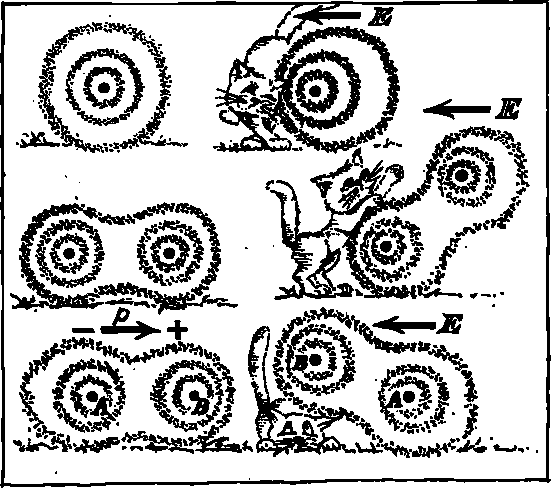
\includegraphics[width=\textwidth]{figures/fig-02-02.pdf}
\caption{Polarization effect of electric field on atoms and molecules.}
\label{fig-2.2}
\end{figure}

The middle drawing illustrates the behaviour of a symmetric diatomic molecule. In the absence of a field it has no moment. The field induces an electric moment. This moment may vary in magnitude in accordance with the angle of the molecule with respect to the field. The moment is formed due to the deformation of the electron shells.

Finally, the lower drawing shows the behaviour of a molecule which has a dipole moment even when there is no field. In our case, the molecule was simply turned when a field was applied. In the general case, however, both mechanisms of polarization are found in substances whose molecules have a dipole moment in the absence of a field: in addition to rotation of the molecule its electrons may also be displaced. These two effects can be readily distinguished by making measurements at very low temperatures where the thermal motion has practically no influence on the molecules.

If our model is valid, we should observe no temperature dependence in the permittivity of substances having symmetric molecules, for example, molecules of oxygen or chlorine. On the other hand, if the diatomic molecule consists of two different atoms, for instance, a molecule of carbon monoxide (\ce{CO}), the permittivity E should be temperature-dependent. This is actually the case. Nitrobenzene is one of the substances whose molecules have a very high dipole moment.

What will happen to ordinary dielectrics when the strength $E$ of the applied electric field is increased? Evidently, the polarization of the substance is increased as well. This takes place due to stretching of the dipoles: in an atom this is a displacement of the electron cloud with respect to the nucleus; in a molecule it may be due to the pulling apart of two ions. This naturally poses the question: Up until what point does an electron, pulled far away from the nucleus by the applied field, remain an electron of the given atom, or do two ions, pulled sufficiently far apart, still form a molecule? Such a limit doubtlessly exists, and, at a sufficiently high field strength, or intensity, $E$, the so-called breakdown of the dielectric occurs. The order of magnitude of this field intensity is several thousand kilovolts per metre. In any case, such breakdown implies the release of electrons or ions, i.e. the production of free current carriers. The dielectric ceases to be a dielectric; it conducts electric current.

We most frequently find such a breakdown when a capacitor is disabled in a television or radio set. We can, however, observe another kind of breakdown: an electric discharge in a gas. Electric discharges in gases are to be specially discussed later. For the present, we shall become acquainted with two distinguished members of the family of dielectrics: piezoelectric and ferroelectric crystals.

Quartz is the chief representative of the class of piezoelectric crystals. Members of this class (which includes, besides quartz, such substances as sugar and tourmaline) must have a definite symmetry. Shown in \figr{fig-2.3} is a crystal of quartz. The principal axis of this crystal is a threefold symmetry axis. Three twofold symmetry axes lie in a perpendicular plane.

\begin{figure}[!ht]
\centering
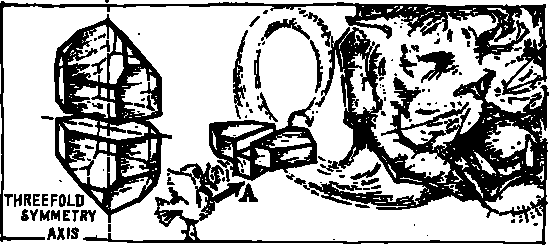
\includegraphics[width=\textwidth]{figures/fig-02-03.pdf}
\caption{Quartz a piezoelectric crystal.}
\label{fig-2.3}
\end{figure}

A plate about \SI{2}{\centi\meter} thick is cut out of this crystal as shown in the drawing. We see that it is perpendicular to the principal axis and that the twofold symmetry axes lie in a plane of this plate. Then a thin wafer, about \SI{0.5}{\milli\meter} thick, is cut out of the thick plate in a direction perpendicular to one of the twofold symmetry axes. Interesting experiments can be conducted with the thin piezoelectric wafer obtained in this manner (it is shown displaced downward in the drawing in the middle of \figr{fig-2.3}).

Let us compress the wafer in the direction of arrow $A$, perpendicular to the symmetry axes, and connect an electrometer (an instrument used to detect electric charges) to the side surfaces of the wafer. These surfaces, actually faces of the wafer, must be silver-plated to ensure proper electric contact. We shall find that compression has induced unlike charges on the faces of wafer. If tension is applied instead of compression, the signs of the charges are reversed: where a positive charge appeared in compression, a negative charge appears in tension and vice versa. This phenomenon -- the induction of electric charges by applying pressure or tension -- is called \emph{piezoelectricity}.

Piezoelectric quartz crystal devices are exceptionally sensitive: electric devices enable us to measure charges induced on the quartz by extremely low forces that could not be measured in any other way. A piezoelectric quartz crystal is also capable of detecting extraordinarily rapid variations in pressure, a feature unattainable with other instruments. Consequently, the effect. described above is of immensely practical significance as a method of electrically detecting all kinds of mechanical action, including sounds. It is sufficient to blow softly at a piezoelectric quartz wafer, and the electric indicating instrument instantly responds.

Piezoelectric quartz wafers are used in medicine to listen to murmurs of the heart. They are also employed in a similar manner in engineering to test the operation of machinery in which they can detect all ``suspicious'' noises.

Quartz is used as a source of the piezoelectric effect in the tone arms (pickups) of record players. The motion of the needle in the groove of the record leads to compression of the piezoelectric crystal, which, in turn, produces the electric signal. The electric current is amplified and is fed to a dynamic loud-speaker to be converted into sound.

So far we have discussed substances that are electrically polarized by an electric field and (in certain cases) by mechanical deformation. When the external effect is
removed, the substance becomes electrically neutral again. But, along with this widespread behaviour, we find certain bodies possessing a total electric moment in the absence of external forces. We obviously cannot find such substances among liquids and gases because thermal motion, which is not withstood by the ordering effect of a field, must inevitably lead to disorder in the arrangement of the dipole molecules. Crystals, however, can be conceived of in which the atoms are arranged so that the centres of gravity of the anions and cations within each unit cell are identically displaced. Then all the dipole moments face the same direction. Such substances could be expected to possess maximum possible polarization and, consequently, a permittivity of huge value.

Such crystals do exist. The phenomenon was first discovered using Rochelle salt and this class of substances are called \emph{ferroelectrics} (or \emph{ferroelectric crystals}).

Of greatest practical value among the ferroelectrics is barium titanate. Using it as an example, we shall discuss the exceptionally singular behaviour of this class of substances.

The unit cell of a barium titanate crystal is illustrated in \figr{fig-2.4}. We have chosen the barium atoms for the corners of the cell. The small light-coloured spheres are anions of oxygen, and the large sphere in the centre is a cation of titanium.

\begin{figure}[!ht]
\centering
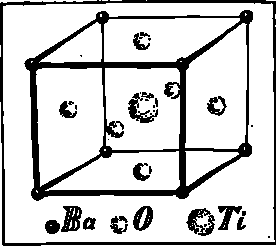
\includegraphics[width=0.4\textwidth]{figures/fig-02-04.pdf}
\caption{The unit cell of a barium titanate crystal.}
\label{fig-2.4}
\end{figure}

The drawing looks as if the cell were a cubic one. A strictly cubic cell of the substance actually does exist, but only at temperatures above \SI{120}{\celsius}. Obviously, a strictly cubic cell is symmetrical and can have no dipole moment. Consequently, the special properties of barium titanate disappear above this temperature, which is called the \emph{Curie point}. Above this temperature the substance behaves as an ordinary dielectric.

When the temperature is lowered below \SI{120}{\celsius}, the ions of oxygen and titanium are displaced in opposite directions by an amount of the order of \SI{0.1}{\angstrom}. At this, the cell acquires a dipole moment.

Note the following especially important fact. This displacement can with equal success take place in any of three directions: along the three axes of the cube. Displacement leads to distortion of the cell. Hence, not all ways of dividing up the crystal regions within which all the dipole moments are arranged in a single direction turn out to be equally expedient.

Feasible ways of dividing a crystal into ideally polarized regions (called domains) are shown in \figr{fig-2.5}.

\begin{figure}[!ht]
\centering
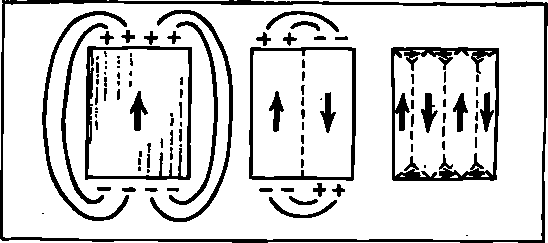
\includegraphics[width=\textwidth]{figures/fig-02-05.pdf}
\caption{Feasible ways of dividing a crystal into ideally polarized regions.}
\label{fig-2.5}
\end{figure}

Along with the case in which the whole crystal is a single domain -- when the maximum electric field is obtained -- there may be less expedient versions and even one (at the extreme right) in which the external field equals zero.

How does a ferroelectric behave when an external field is applied to it? It was found that the polarization mechanism consists in the growth of a domain that faces the ``required'' direction. by spreading its boundaries. Domains oriented with their dipole moment at an acute angle to the field ``devour'' domains oriented at an obtuse angle. When located in very strong fields, inversion of the: domains may also be observed.

Barium titanate is the main industrial ferroelectric. It is obtained by the firing of two powders: titanium dioxide and barium carbonate. The result is a kind of ceramic material.

Ceramic ferroelectrics are extensively applied in electrical and radio engineering. Their main feature is that they drastically increase the permittivity of capacitors. Moreover, as is clear from the described polarization mechanism, the value of $\varepsilon$ increases with the intensity of the electric field. A capacitor is thus converted into a varactor, or variable capacitor, by means of which frequency modulation can be most easily accomplished. This is a process that takes place in any radio or TV set.

For many purposes, ferroelectric ceramics have replaced quartz. They can be used to produce more powerful sounds. In the same way, the gain is higher for ultrasounds as well. The only field in which quartz has no competitors is the stabilization of radio frequencies.

The great majority of textbooks begin their chapters on electricity by describing electric charges produced on glass or hard rubber rods by rubbing them. The explanation of this phenomenon is usually evaded. Why?

First we should emphasize the fact that the electrification of dielectrics by friction is not related (at least, directly) to the polarization of insulators that we have just discussed. As a matter of fact, polarization consists in the formation of bound electric charges whose special feature is that they cannot be ``drawn off'' the dielectric. The charges produced on the glass or hard rubber by rubbing them with cat fur are obviously free charges and, of course, that means electrons.

The general picture of what takes place is more or less clear, but not entirely. Apparently, the scanty amount of free electrons possessed by the insulator are bound to its molecules by forces of various magnitudes for various dielectrics. Hence, if two bodies are held in tight contact, electrons may pass over from one to the other. At this, electrification occurs. But tight contact here means to bring the surfaces within distances equal to interatomic ones. Since no atomically smooth surfaces exist in nature, rubbing helps to eliminate all kinds of projections and increases the area, so to say, of true contact.

Transfer of electrons from one body to another may occur for any pair of bodies, whether they are metals, semiconductors or insulators. But only insulators (or nonconductors) can be electrified because only in such bodies do the charges remain at the places to which they were rubbed off the other body.

I cannot express especially full satisfaction with this theory. It does not explain the advantages of using hard rubber, glass and cat fur for this purpose. We can pose heaps of more questions that have no convincing answers.

\section{Conduction in Gases}

If we fill a glass tube with a gas, seal electrodes into the tube and apply a voltage across them, we obtain a simple device for studying the conduction of electricity in gases. We can change the substance through which the current passes, we can vary the pressure of the gas and the applied voltage.

\begin{figure}[!ht]
\centering
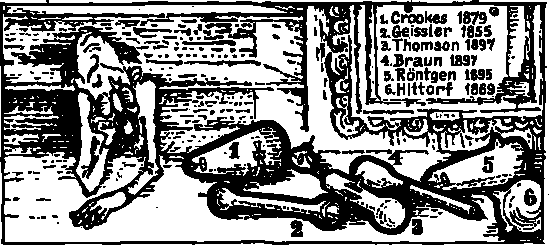
\includegraphics[width=\textwidth]{figures/fig-02-06.pdf}
\caption{Various shapes of tubes devised for studying conduction of gases.}
\label{fig-2.6}
\end{figure}

Investigations of the conduction in gases played an immense role in developing our concepts of the electrical structure of matter. The main part of this research was conducted in the nineteenth century.

Tubes of various shapes, used to study the phenomena we are discussing, are illustrated in \figr{fig-2.6}. Since all ancient statues and paintings of the old masters have long since been purchased and repurchased, dealers in antiques are now offering connoisseurs obsolete laboratory equipment. In curiosity shops in Western Europe and America, you can buy (usually at a good price) one of the rare items shown in \figr{fig-2.6}.

An electric current is initiated in a gas because the neutral molecules are broken down into anions and cations. Moreover, an electron may break away from molecules and atoms. The current is produced by a beam of positive ions and beams of negative ions and electrons travelling in the opposite direction.

To make a gas conduct a current it is necessary to convert the neutral molecules or atoms into charged particles. This may be accomplished either by an external ionizer, or by collision of the particles. As mentioned above, external means of ionization may be ultraviolet, $X$-, cosmic or radioactive rays. High temperature also leads to the ionization of a gas.

The passage of a current through a gas is often accompanied by some light effect. The character of the glow varies with the gas used, its pressure and the voltage applied. Investigations of this glow played a vital role in the history of physics, particularly as a source of information on the energy levels of the atoms and the
laws of electromagnetic radiation.

Conduction in a gas does not obey Ohm's law. It is characterized by a curve showing the dependence of the current on the voltage. This curve is called the \emph{current vs voltage characteristic} (not only for gases, but for any conducting systems that do not conform to Ohm's law).

Let us consider the phenomena, typical of any gas, that occur when voltage applied to a gas-discharge tube is increased. This behaviour of the gas, now to be described, is found in a wide pressure range. We shall except only such low pressures for which the free path of the molecules becomes commensurate with the dimensions of the gas-discharge tube. Our discussion will also not refer to such high pressures at which the density of gases approaches that of liquids.

We begin by applying a low voltage across the tube. If we do not use some ionizer, there is no current through the tube. If an ionizer is available, it produces charged particles -- ions and electrons -- in the gas. As soon as a field is set up in the tube, the particles are directed by the field to the electrodes of the tube. The velocity at which the charged particles travel toward the electrodes depends upon many circumstances and primarily on the field intensity and gas pressure.

Chaotic motion is superimposed on the ordered motion of the ions and electrons resulting from the constant electric force. A particle accelerated by the field travels only a short distance. Its short run inevitably ends in a collision. At low velocities, these collisions conform to the law of elastic collisions.

The mean free path is determined first of all by the pressure of the gas in the tube. The higher the pressure, the shorter the mean free path and the lower the average velocity of ordered motion of the particles. Voltage applied across a gas-discharge tube has the opposite effect: higher voltage raises the average velocity of ordered motion of the particles.

If no voltage is applied across the tube, the following events occur in the gas. The ionizer produces ions and then ions of opposite signs join each other when they meet. This is called ion recombination. Since it takes a pair of particles to recombine, the rate of this process is proportional to the square of the number of particles.

When the ionizer operates continuously, equilibrium is set up between the two processes: ionization and recombination. This is what happens in the ionosphere surrounding our earth. Depending upon the time of day and the season, the number of ionized particles in a cubic centimetre varies from a million to hundreds of millions of ions and electrons. Thus, the degree of ionization is a quantity of the order of one per cent (recall the number of air molecules in unit volume at high altitudes).

But let us return to the ionized gas in the tube subject to a voltage. Equilibrium is upset, of course, between ionization and recombination because a part of the ions reach the electrodes before they are recombined. As the voltage is raised, a larger and larger part of the ions produced in unit time reach the electrodes, increasing the current through the gas. This continues until there is no time left for recombination and all the ions produced by the ionizers reach the electrodes. It is obvious that no further increase in voltage can increase the current (this is called the \emph{saturation current} and is represented by the horizontal portion of the current-voltage characteristic in \figr{fig-2.7}).

\begin{figure}[!ht]
\centering
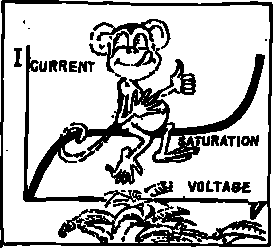
\includegraphics[width=0.4\textwidth]{figures/fig-02-07.pdf}
\caption{Current-voltage characteristics of a gas discharge tube.}
\label{fig-2.7}
\end{figure}

The less the density of the gas, the lower the field voltage at which the saturation current is reached.

The saturation current is equal to the charge of the ions formed by the ionizer in one second throughout the volume of the tube. The saturation current is usually not very large: of the order of a microampere or less. Its magnitude depends, of course, on the number of destructive missiles with which the ionizer bombards the gas.

When we operate the tube at a point on the current-voltage characteristic within the limits of the saturation current and protect the gas from the effects of an external ionizer, the current ceases to flow. This is said to be a non-self-maintained gas discharge.

If the voltage is raised again, new phenomena occur. At a certain instant, the velocity of the electrons becomes high enough for them to knock electrons out of the neutral atoms and molecules. For this the voltage across the tube should reach a value at which an electron acquires energy sufficient in its free path to ionize a molecule. The initiation of collision ionization has a marked effect on the current-voltage characteristic: the current begins to increase again because an increase in voltage leads to an increase in the velocity of the electrons. An increase in velocity, in its turn, raises the ionizing capacity of the electrons so that a greater number of ion pairs is produced and the current increases. The current-voltage characteristic curve turns sharply upward. In comparison with the saturation value, the current increases by hundreds and thousands of times and the gas begins to glow.

Now, if we eliminate the action of the external ionizer, the current continues to flow. We have gone over to the region of a self-maintained gas discharge. The voltage at which this qualitative change occurs is called the \emph{breakdown voltage} or the \emph{ignition voltage of a gas discharge}.

The sharp increase in current in passing over this critical limit is due to the avalanche-type increase in the number of charges. One released electron destroys a neutral molecule and produces two charges of such high energy that they are capable of breaking down another pair of molecules that they encounter. Thus, two charges form four, four form eight, etc. You must agree that the use of the word ``avalanche'' is fully justified. 

A quantitative theory has been proposed that predicts the shape of the current-voltage characteristic curves for gases with a fair degree of accuracy.

\section{Self-Maintained Discharge}

There are many types of discharges in gases. We shall discuss only a few.

\noindent\hlgray{{\grotsq Spark discharge.}} A spark passing through the air between two electrodes can be readily observed in the most elementary experiments. Sparks can be produced simply by bringing two wires, across which a voltage has been applied, sufficiently close together. What do we mean by ``sufficiently''? If air is the medium through which the spark is to pass, the required field intensity is 30 thousand volts per centimetre. This means that a potential difference of 3000 volts is sufficient for a small gap of one millimetre. Any reader has observed such small sparks in everyday life when repairing faulty electric wiring or when bringing two leads from the terminals of a storage battery close together (here the gap between the ends of the leads must equal the thickness of a safety razor blade).

The breakdown voltage depends upon the density of the gas. It also depends upon the shape of the electrodes. A spark can pass through dielectric liquids and solids as well as through a gas. It is important for an electrician to know the breakdown voltage of all the materials he uses in his work.

Today it seems quite obvious to us that lightning is a spark jumping between clouds charged with electricity of opposite sign. This was not always the case, however, and Mikhail Vasilievich Lomonosov (1711-1765) and Benjamin Franklin (1706-1790) made great efforts to prove this statement. Georg Wilhelm Richmann (1711-1753), a Russian physicist that collaborated with Lomonosov, lost his life in an attempt to ground lightning through a twine that conducted electricity from a kite that he flew during a thunderstorm.

Interesting data are available on the spark discharge in a bolt of lightning. The voltage between the cloud and the earth is about \num{d8} to \num{d9} volts and the current ranges from tens to hundreds of thousands of amperes. The diameter of the spark channel ranges from 10 to \SI{20}{\centi\meter}.

The duration of a flash of lightning is extremely short: of the order of 8 microsecond. We can readily estimate that the quantity of electricity passing through the lightning channel is comparatively small.

These sparks from the heavens have been studied in detail by means of high-speed motion picture photography. A bolt of lightning quite frequently consists of a series of spark discharges following a single path. Lightning has a sort of ``leader'' which pierces the most convenient, always freakishly branched way for the electric discharges.

Also observed to some extent is ball lightning. This type is not fully understood and cannot, unfortunately, be reproduced under laboratory conditions. It is an incandescent sphere of gaseous plasma, 10 to \SI{20}{\centi\meter} in diameter. Ball lightning moves slowly and is sometimes even stationary. It exists several seconds, or even minutes, and then disappears with a powerful explosion. It must be admitted that so far no comprehensive theory of this interesting phenomenon has been proposed.

\noindent\hlgray{{\grotsq Arc discharge.}} An arc discharge was first obtained by the famed Russian physicist and electrical engineer Vasily Vladimirovich Petrov (1761-1834) as far back as 1802. He struck the arc by bringing into contact two pieces of carbon across which a powerful voltage had been applied from a source of electric energy. Then he moved the carbons (electrodes) apart. This procedure is still being employed today. True, special carbon rods of pressed graphite powder are used as the electrodes. The positive rod burns away more rapidly than the negative
one. By just looking at the electrodes we can immediately find to which one the positive pole is connected: a hollow, called the crater, is formed at its end. The temperature in the crater at standard pressure may reach \SI{4000}{\celsius}. If the pressure is increased, the temperature can be raised almost \SI{6000}{\celsius}, i.e. the temperature at the surface of the sun. An arc struck between: metal electrodes has a flame with a considerably lower temperature.

A low voltage, of the order of 40 to 50 volts, is sufficient to maintain the arc. The current may reach hundreds of amperes because the resistance of the incandescent gaseous column is low.

How do we explain the high electrical conductivity of the gas at such low voltages? The molecules are not accelerated to high velocities, and their collisions cannot play much of a role in producing a heavy current, The explanation is as follows: at the first instant the arc is struck, a large quantity of heat is evolved at the point of contact, drastically raising the temperature at the ends of the electrodes. This initiates the process of thermal electron (thermionic) emission in which the cathode ejects an immense number of electrons. From this it follows, by the way, that only the high temperature of the cathode is of importance; the anode can remain cold.

The mechanism of an arc discharge of this type is entirely different from that of a spark discharge.

No need, evidently, to remind the reader how important this phenomenon is in engineering practice. Arc discharges are widely employed in welding and cutting metals, as well as in electrometallurgy.

\noindent\hlgray{{\grotsq Glow discharge.}} This kind of self-maintained discharge is also of great practical value, since it takes place in gas-discharge tubes or, as they are also called, daylight lamps. The tube is designed and is filled with gas
(at a pressure substantially below atmospheric pressure) so that it operates at a voltage exceeding the ignition voltage. The electric current in gas-discharge lamps is produced by the ionization of the gas molecules by electrons, and also because electrons are knocked out of the cathode. A gas-discharge lamp does not ignite instantaneously. This is evidently due to the fact that the first impulse must be obtained from the small amount of charged particles that are always present in any gas.

\noindent\hlgray{{\grotsq Corona discharge.}} A corona is observed at atmospheric pressure in a highly nonuniform field, for example, in the vicinity of a wire or sharp point. The field intensity should be high: of the order of a million volts per metre. It makes no difference to which pole the sharp point is connected. Thus, there are both positive and negative coronas. Since the field intensity is reduced as we depart from the sharp point, the corona disappears at a short distance away. We can contend that a corona discharge is an incomplete breakdown of the gas gap. A corona is produced by electron avalanches travelling either toward the point or from the point to external space. Besides electrons, the corona region contains negative and positive ions -- products of disintegration of the neutral air molecules. The corona glows only in the small space near the point in which there is an electron avalanche.


The initiation of a corona depends on the atmospheric conditions and, primarily, the moisture.

The atmospheric electric field may cause the tops of trees and tips of ship's masts to glow. Formerly, this phenomenon was called St. Elmo's fire. It was supposed to be an evil omen. This has a reasonable explanation. It may well be that such a glow is observed just before a storm breaks.

We can learn a moral lesson from an event that took place quite recently. Two amateur investigators, Mr. and Mrs. Kirlian, had spent some years studying the following phenomenon. A person lays a hand, connected to one terminal of a high-voltage power supply, on a photographic film that is separated by a layer of insulation from the other electrode of the same power circuit. When the voltage is switched on, a blurred image of the palm and fingers is obtained on the film. This image is due to a corona discharge. Naturally, the voltage must be less than that required for a spark breakdown of the insulation.


These experiments drew the attention of experts in the field of so-called parapsychology, the general name for a group of ``theories'' that the great majority of physicists and psychologists consider to be pseudo-scientific.
This attention was due to the fact that the Kirlians and their followers related the kind of photograph obtained to the ``psychic'' state of the subject.

As a result of the extensive publicity received by such an extravagant interpretation of these experiments, a group of physicists and psychologists from various universities in the USA decided to check the experiments more carefully. They searched for a simpler explanation of the undoubted fact that the appearance of the photograph thus obtained really does differ for different persons or even for the same person if the photograph is taken under different conditions.

The investigators reached the following conclusion: ``Photographic images obtained by the Kirlian technique are principally a record of corona activity during an exposure interval. Most of the variations in the images of the corona of a living subject who is in contact with the photographic film can he accounted for by the presence of moisture on or within the subject's surface. During exposure, moisture is transferred from the subject to the emulsion surface of the photographic film and causes an alteration of the electric charge pattern on the film, hence the electric field at the surface of the subject.''

The investigators proposed further application of this technique, which they preferred to call ``corona-discharge photograph'', ``for the detection and quantification of moisture in animate and inanimate specimens through the orderly modulation of the image due to the various levels of moisture.''

This interesting piece of information, published in the December 1976 issue of the journal \emph{Scientific American} with the title ``Sweaty Palms'', leads to two conclusions. In the first place, any real phenomenon deserves attention and it is quite possible that it may prove useful in practice. Secondly, when an investigator discovers a new fact, he should begin by overcoming the temptation to interpret it in a way that does not fit in with up-to-date scientific concepts. The discovery can be made public and presented for judgement by specialists only after it has been comprehensively shown that existing theories are incapable of explaining the new fact.

Real facts, which are falsely interpreted and explained, can be called (after an old joke) cockroach experiments. According to the joke, the legs are pulled off one cockroach which is then placed on a table side by side with a cockroach having all his legs. The ``investigator'' then knocks on the table. The uninjured cockroach runs away while the ``cripple'' remains. This proves, contends the ``investigator'', that a cockroach hears with its legs.

Every year publications appear that describe such ``cockroach experiments''. I consider it good policy to warn my readers against them.

\section{Matter in the Plasma State}

The term Plasmenzustand was proposed as far back as 1939 by two German scientists whose article was translated into the Russian by the author for the Soviet journal \emph{Advances in Physical Sciences}. This seems to be a suitable name. As a matter of fact, plasma is neither a solid, nor a liquid, nor a gas. It is a special state of matter.

Thermal ionization of gases, i.e. stripping the atoms of their electrons and the disintegration of neutral molecules into ions, begins at temperatures exceeding 5 or 6 thousand degrees. Is it worthwhile, then, to discuss this problem? No materials exist that can withstand a higher temperature.

It certainly is worthwhile! The great majority of celestial bodies, like our sun, are in a plasma state. An example of plasma is the ionosphere. Plasma can be confined in a limited volume by properly shaped magnetic fields, so-called magnetic bottles, under laboratory conditions. We can, in addition, speak of the plasma of a gas discharge.

The degree of ionization of a gas depends on the pressure as well as the temperature. Hydrogen at a pressure of the order of \SI{1}{\milli\meter} of mercury column is practically completely ionized at a temperature of 30 thousand degrees. Under such conditions, there is only one neutral atom per 20 thousand charged particles.

Hydrogen in the plasma state consists of a mixture of chaotically travelling and colliding particles of two gases: proton ``gas'' and electron ``gas''. Plasma formed of other substances is a mixture of many ``gases''. In such a plasma we find electrons, bare nuclei, various ions, as well as a negligible quantity of neutral particles.

A plasma with a temperature of tens or hundreds of thousands of degrees is said to be cold. A hot plasma has a temperature of millions of degrees.

But one must be careful with the concept of a plasma temperature. As the reader knows, temperature is uniquely determined by the kinetic energy of the particles. In a gas consisting of heavy and light particles, a state of equilibrium is set up only after the heavy and light particles have acquired the same average kinetic energy.

This means that in a gas existing for some time under stable conditions, the heavy particles travel slowly and the light particles, rapidly. The time required to set up equilibrium depends on what we had ``at the beginning''. Other conditions being equal, the greater the difference between the masses of the particles, the longer the time required to attain equilibrium.

These are exactly the conditions we find in a plasma. The mass of the lightest nucleus is almost two thousand times greater than that of an electron. In each collision, an electron transmits only a small part of its energy to a nucleus or ion. Thus the average kinetic energies of all the particles of plasma are equalized only after an immense number of collisions. Such a plasma is said to be \emph{isothermal}. It is the kind existing in the interior of the sun and other stars. The time required to reach equilibrium in a hot plasma ranges from fractions of a second to some seconds.

The plasma in a gas discharge (spark, arc, etc.) is a different matter. Here the particles not only travel chaotically, but also produce an electric current. In their path between the electrodes, the rapid electrons do not have the opportunity to transmit any appreciable part of their energy to the leisurely paced ions. This is why the average velocity of the electrons in a gas discharge is much higher than that of the ions. Such a plasma is said to be \emph{nonisothermal} and must be specified by two temperatures (or even three if we take the neutral particles into account). Naturally, the electron temperature is substantially higher than the ion temperature. Thus, in an arc discharge, the electron temperature is from 10 to 100 thousand degrees, while the ion temperature is close to 1000 degrees.

The behaviour of the particles in a plasma can be described by means of the same quantities that are used in the kinetic theory of gases. Many techniques have been devised for directly or indirectly determining the mean free path of the particles, the mean free time, and the concentrations of particles of various kinds.

To provide the reader with an idea of the orders of magnitude found in plasma physics, we present certain data describing a high-concentration hydrogen plasma (\num{d20} ions per cubic metre). It was found that in a cold plasma (at a temperature of \SI{10000}{\celsius}), the mean free path equals \SI{0.03}{\centi\meter} and the mean free time is \SI{4d-10}{\second}. If the same plasma is heated to a hundred million degrees, the respective figures are \SI{3d6}{\centi\meter} and \SI{4d-4}{\second}.

In citing such data, it is absolutely necessary to specify additionally the kind of collisions we have in mind. The data given are for encounters between electrons and ions.

It is evident that a volume containing many particles is electrically neutral. But we may be interested in the behaviour of the electric field at some definite point in space. The field varies rapidly and drastically because ions and electrons alternate in rushing past the point. The rapidity of these variations can be calculated, as can the average intensity of the field. Plasma complies with the condition of neutrality with exceptionally high precision. Strictly speaking, we should employ the term ``quasi-neutrality'', i.e. near-neutrality. But what do we mean by this ``near''?

Rather simple calculations indicate the following. Consider a length of one centimetre in the plasma. Calculate the electron and ion concentrations for each point in this length. Quasi-neutrality means that these concentrations should be ``nearly'' equal. Next, let us imagine that in one cubic centimetre we have an ``extra'' amount of electrons that are not neutralized by positive ions. If this is so and the particle density is equal to the air density at the earth's surface, a field with an intensity of about \SI{1000}{\volt\per\centi\meter} is set up along the length being considered, even if the difference in ion and electron concentrations equals only one thousand millionth of one per cent! Here is what the word ``near'' signifies.

But even this negligible lack of equality of positive and negative charges lasts only for an extremely short instant. The field that forms excludes all the superfluous particles. This automatism is already operable for regions measured by thousandths of a centimetre.

We shall return to plasma in magnetic bottles again in Book~4. The reader has undoubtedly seen accounts, and perhaps descriptions, of installations of the Tokomak type (in the USSR). A whole army of scientists are working on their improvements. The point is that if a high-temperature plasma could be produced and properly handled, it would lead to controlled fusion of light atomic nuclei, which would be accompanied by the generation of titanic amounts of energy. Physicists have learned to realize this process (uncontrolled fusion) in bombs. Will it be possible to produce a plasma with a sufficiently high temperature and sufficiently long duration to initiate a chain reaction of the kind accomplished in a nuclear reactor? There is no answer yet to this question.

\section{Metals}

The subdivision of solids into various classes according to their electrical resistance is based on the mobility of their electrons.

An electric current is a stream of moving charged particles. When we deal with streams of ions or electrons, we literally visualize an electric current. An electric current also reveals itself distinctly in passing through liquids because matter is deposited on the electrodes. But as for solids, there is only circumstantial evidence of the passage of an electric current.

A series of facts are available that enable us to make the following statements. No displacement of the atomic nuclei occurs in solids. An electric current is produced by electrons. The electrons travel due to the energy supplied by the current source. This source sets up an electric field inside the solid.

The equation relating the voltage and the electric field intensity is valid for any conductors. Therefore, combining the equations on page \pageref{curr-density} and \pageref{energy-field}, we can write Ohm's law for a solid conductor in the form
\begin{equation*}%
j= \sigma E
\end{equation*}
where $\sigma =1/\rho$ is called the \emph{electrical conductivity}. 

The electrons of a solid can be divided into bound and free electrons. The bound electrons belong to definite atoms; the free electrons form a kind of electron gas. These electrons move around in the solid. When no voltage is applied to the solid, the electrons have random motion. The more the motion of the free electrons is impeded, the oftener they collide with fixed atoms and with one another, the higher the electrical resistance of the body. 

The vast majority of electrons in a dielectric have an owner that is either an atom or a molecule. The number of free electrons is negligible.

In metals each atom donates one or two electrons for common use. This electron gas is the current carrier. On the basis of a roughly approximate model we can estimate the electrical conductance and thereby check the model.

In exactly the same way as when we discussed a molecular gas, we shall assume that each electron manages to travel a path of length $l$ without collisions. The distance between the atoms of a metal equals several angstroms. It is logical, then, to assume that in order of magnitude the mean free path of the electrons equals \SI{10}{\angstrom}, i.e, \SI{d-7}{\centi\meter}.

In its motion the electron is subject to the accelerating force $eE$ during the time $l/v$, where $v$ is its velocity. The chaotic velocity of electrons can be estimated on the basis of data obtained in investigations of thermionic (thermal electron) emission. This velocity is of the order of \SI{d8}{\centi\meter\per\second}.

To determine the velocity of ordered motion of electrons, i.e. the velocity of the motion that produces a current, the acceleration $eE/m$. is to be multiplied by the mean free time. This assumes that each collision discontinues motion of the electron, after which it begins to pick up speed again. Multiplying, we obtain the velocity of the electrons that produce the electric current:
\begin{equation*}%
u= \frac{eEl}{mv}
\end{equation*}
Next, we attack the problem of determining the resistivity of a metal. If we obtain the correct order of magnitude, then we can presume that our model ``works''.

We shall leave to our readers the task of showing that the current density $j$ can be written as the product of the number of electrons in unit volume by the charge of the electron and by the velocity of ordered motion (drift) of the electrons. Thus $j=neu$. Substituting into this equation the drift velocity, we obtain 
\begin{equation*}%
j = \frac{ne^{2}l}{mv}E
\end{equation*}
Then the electrical conductivity is
\begin{equation*}%
\sigma = \frac{ne^{2}l}{mv}
\end{equation*}
If we assume that each atom contributes one electron for common use, then we find that a conductor has a resistivity of the order of \SI{d-5}{\ohm\meter}. A very reasonable value! It confirms both the validity of our roughly approximate model and the proper choice of the values of the parameters in our ``theory''. I place the word theory in quotation marks only because it is a crude approximation and elementary. This example, however, illustrates the typical physical approach in interpreting phenomena.


According to the theory of a free electron gas, the electrical resistance should decrease with a drop in temperature. But do not hasten to relate this circumstance with the change in the velocity of chaotic motion of the electrons. This velocity has nothing to do with the matter because it depends only slightly on the temperature. The reduction in resistance is due to the reduced amplitude of vibration of the atoms. As a result, the mean free path of the electrons increases.

This fact can also be expressed in other words: upon an increase in the amplitude of vibration of the atoms, the electrons are scattered to a greater degree in various directions. Consequently, the component velocity in the direction of the current is reduced, i.e. the resistance should increase.

The increase in electron scattering also explains the increased resistance of a metal (and not only a metal) when impurities are added to it. The impurity atoms act like defects in crystal structure and therefore facilitate electron scattering.

Electric energy, as we know, is transmitted by wires. Owing to their resistance, the wires draw energy from the current source. Such energy losses are enormous and their prevention is one of the most vital of engineering problems.

There is hope that this problem can be solved on the basis of the remarkable phenomenon known as \emph{superconductivity}.

In 1911, the Dutch physicist Heike Kamerlingh Onnes (1853-1926) found that at temperatures close to absolute zero certain bodies suddenly lose practically all of their electrical resistance. If a current is induced in a ring-shaped superconductor, it continues to flow for days without diminishing. Of pure metals, the highest temperature at which superconductive properties are found is about \SI{9}{\kelvin}, the metals being niobium (\SI{8.9}{\kelvin}) and technetium (\SI{9.3}{\kelvin}). No need to mention what a vast army of scientists are engaged in the search of superconductors that would acquire this wonderful property at a higher temperature. So far they have not been any too successful, though an alloy has been discovered that is claimed to become superconductive at about \SI{20}{\kelvin}.

There is reason to believe, however, that this limit can be raised (perhaps even to room temperature). The search is being made among special polymer substances and among complex lamellar materials in which a dielectric alternates with a metal. The significance of this problem can hardly be overvalued. I take the liberty of regarding it to be one of the cardinal problems in modern physics.

The search for superconductors that acquire this property at sufficiently high temperatures especially gained in scope after a theory had been proposed for this phenomenon. This theory suggested new courses along which the required materials might he found.

It is characteristic that much time passed between the discovery of the phenomenon and its explanation. The theory was advanced in 1957. It might be well to point out that the laws of quantum physics, on which the theory of superconductivity is based, were established as far back as 1926. It follows that the explanation of the phenomenon is far from simple. In this book I can only start, as you might say, from the middle of the story. It seems that with the slowing down of vibrations in the atomic lattice, certain electrons become ``paired''. Such a ``pair'' behaves in coordination with each other. When the pairs are scattered by the atoms (and this scattering, as mentioned above, is the cause of resistance), the rebound of one of the members of the pair to one side is compensated for by the behaviour of its ``friend''. This compensation is in the sense that the total momentum of the electron pair remains constant. Thus, electron scattering does not disappear but no longer influences the passage of the current.

In addition to paired electrons, a superconductor also carries ordinary electron gas. Hence, two fluids seem to exist simultaneously: one is ordinary and the other is superconductive. As the temperature of the superconductor is raised from absolute zero, thermal motion breaks apart more and more electron pairs, and the percentage of the ordinary electron gas increases. Finally, at the critical temperature, all the paired electrons disappear.

In Book~2 we made use of the two-fluid model, with one-ordinary fluid and one special fluid, to explain superfluidity observed in liquid helium. These two phenomena are closely related: superconductivity is superfluidity of the electron fluid.

Each electron pairs of the kind mentioned above, has a total spin equal to zero. Particles with a spin equal to zero or a whole number (i.e. with integral spin) are called bosons. Under certain known conditions, large amounts of \emph{bosons} can occupy the same energy level. In such cases their motions become ideally coordinated and nothing can impede their displacements. We shall return to this phenomenon again in Book~4.

\section{Electron Emission from Metals}
Since a part of the electrons behaves like a gas of rapid particles, it is natural to expect that electrons are capable of emerging to the surface of a metal. For the electron to leave the metal entirely, it must overcome the attractive forces of the positive ions. The work done by the electron for this purpose is called the \emph{work function}.

The higher the temperature of the metal, the greater the kinetic velocity of the electrons. If the metal is heated to incandescence, an appreciable number of electrons will be able to escape from it.

Thermionic emission, as the ejection of electrons from a metal is called, can be investigated by a simple experiment. An additional electrode is sealed into an electric light bulb. A sensitive instrument can be used to measure the current set up by the part of ``evaporating'' electrons that reach the new electrode (a part, and not all, because the electrons fly out of the incandescent filament in all directions).

To evaluate the work function we resort to a ``barrier'' voltage, i.e. we connect the sealed-in electrode to the negative pole of a battery. Gradually raising the voltage, we reach a value at which the emitted electrons can no longer arrive at the electrode.

The electron work function for tungsten is about 5 electron volts. Special coatings can, if required, reduce the work function to one electron volt.

What is this unit of work called the \emph{electron volt}? It is, as the name implies, the energy acquired by an electron in travelling over a portion of its path with a voltage of one volt applied across this portion. One electron volt equals \SI{1.6d-19}{\joule}. The thermal velocity of electrons is quite considerable, but their mass is very small. Therefore, the given barrier height is extremely large. Theory and experiments show that electron emission depends drastically on the temperature. A temperature rise from 500 to \SI{2000}{\kelvin} increases the emission current a thousandfold.

Owing to thermal motion the emission of electrons from a metal is, so to speak, a natural process. But electrons can also be knocked out of a metal.

In the first place, this can be done by bombarding the metal with other electrons. This is called \emph{secondary} (electron) emission. It is made use of to multiply the number of electrons in certain engineering instruments.

Vastly more essential is the extraction of electrons from solids by light. This phenomenon is called the \emph{photoelectric effect}.

\section{Thermoelectric Phenomena}

Very long ago (in the evolution of mankind this time is a mere instant, but in the development of science it is almost as long as eternity), over 150 years in the past, a simple fact was discovered. If an electric circuit is
made up of a piece of copper wire and a piece of bismuth wire by soldering them together at two junctions, current flows through this circuit. This happens only when the temperature of one junction is higher than that of the other. This is the \emph{thermoelectric effect}.

What makes the electron travel along our combined circuit? The explanation of this phenomenon is not at all simple. The electromotive force is due to two factors. In the first place, we have a contact electric field, secondly, we have a temperature electric field.

We have just mentioned that work is required to remove an electron beyond the limits of a metal. It is natural to assume that work function $A$ differs for various metals. Hence, there is a voltage across the junction of the two metals equal to
\begin{equation*}%
\frac{1}{e} \, (A_{1} - A_{2})
\end{equation*}
\label{work-func}
The contact voltage can be detected experimentally. By itself, however, this voltage cannot set up a current in a closed circuit. Such a circuit obviously consists of two junctions and the contact voltages oppose and cancel each other. But why does the difference in the temperatures of the junctions produce an electromotive force? The answer is the only logical one. Evidently the contact voltage depends upon the temperature. Heating one of the junctions makes the voltages unequal and sets up a current. But here we must take another phenomenon into account. It can naturally be assumed that there is an electric field between the ends of a conductor if these ends have different temperatures because the electrons travel faster at higher temperatures. This being the case, diffusion of the electric charges begins and continues until a field is set up that counteracts the tendency to uniform distribution.

Experiments leave no doubt of the fact that both phenomena are simultaneously present and both are to be taken into account in proposing a theory.

Thermoelectromotive forces are small: of the order of a millivolt for a temperature difference of 100 degrees. Such voltages are readily measured. Consequently, the thermoelectromotive effect is employed for measuring temperatures. You cannot, of course, insert a liquid-in-glass thermometer into molten metal. For such purposes a \emph{thermocouple} (as the thermoelement used for measuring temperatures is called) is an excellent instrument. A thermocouple has, in addition, many other advantageous
features. How vitally important it may be to measure temperatures at great distances. And the exceptional sensitivity. Electrical measurements are always precise, and it was found that differences in temperature as small as a millionth of a degree can be sensed by a thermocouple.

This high sensitivity enables thermoelements to be applied for measuring heat flow from extremely remote objects. The reader can himself estimate the possibilities of a thermoelement. Suffice it to say that a tenth of an erg per second is no limit.

Like storage cells, thermoelements are frequently assembled into banks to form a thermal battery. If the power requirements are not very high, such a battery can serve as a generator of energy and can find application in radio communications.

\section{Semiconductors}

A great many substances, both elements and chemical compounds, have conductivities filling the wide range between conductors and insulators. Such substances were first discovered a long time ago. But a mere twenty years ago it was hardly probable that anyone could foresee that semiconductor physics would give rise to a powerful branch of industry whose importance in world economics cannot be overrated. Without semiconductors, up-to-date electronic computers, TV sets and tape recorders would be unfeasible. Radio engineering is inconceivable today without semiconductors.


Insulators (nonconductors) have a conductivity ranging between \num{d-8} and \SI{d-18}{\per\ohm\per\meter}, the range of conductivity of metals in the same units is from \num{d2} to \num{d4}. The conductivity of semiconductors lies between these two ranges. As we shall see, not only their resistance is of interest in dealing with semiconductors.

Like in metals, no chemical changes occur in semiconductors when we pass an electric current through them. This indicates that the ions of these substances, forming the frame of their crystal lattice, are not moved around by the action of the electric field. Therefore, as in metals, the motions of the electrons are responsible for electric conduction.

Though this seems obvious, physicists, in the early stages of semiconductor research, decided, in any case, to find which charges were the current carriers. For solids, this can be done by means of the \emph{Hall effect}, discovered in 1879 by Edwin Herbert Hall (1855-1938).

In the next chapter I shall remind you that a magnetic field deflects positive and negative particles in different directions. If a solid in which charges are travelling is made in the form of a plate and is placed in a magnetic field of the proper direction, a voltage appears across the edges of the plate. This arrangement is shown schematically in \figr{fig-2.8}.
\begin{figure}[!ht]
\centering
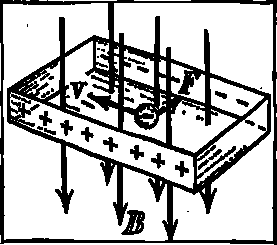
\includegraphics[width=0.4\textwidth]{figures/fig-02-08.pdf}
\caption{The Hall effect in solids.}
\label{fig-2.8}
\end{figure}

The physicists were surprised to find that certain bodies, when investigated in this manner, behaved sometimes as if positive particles were travelling along the conductor, and at other times, as if the carriers of electric charge were negative. We can readily find names for this behaviour. We call the first case positive ($p$-type) conduction and the second, negative ($n$-type) conduction. The point, of course, is not in the name, but in an explanation of the matter. There is no doubt that electrons are travelling inside the semiconductor. How can we reconcile this contradiction? How can we explain the positive conduction?

Imagine a formation of athletes. For some reason, one man drops out of line. This leaves an empty space. Though it doesn't sound any too aesthetic, we can say that a
``hole'' is formed. To dress the ranks, the commanding officer tells the neighbour of the ``hole'' to move over one place. It is absolutely clear that this forms a new empty space. It can be filled by commanding the next man to move into the ``hole''. If the athletes shift, one by one, to the left, the ``hole'' moves to the right. This is the mechanism that explains positive conduction of semiconductors.

The concentration of free electrons is very low in semiconductors. Hence, the definition itself of conduction (recall the formula we derived a few pages back for the current density) should suggest that the majority of atoms in a semiconductor are not in the form of ions, but are neutral atoms. Still, a semiconductor is not an insulator. Consequently, a small number of electrons are freed. These electrons travel as in a metal and are responsible for the negative, i.e. electron, conduction. But a positive ion, surrounded by neutral atoms, is in an unstable state. As soon as an electric field is applied to the solid, a positive ion tries to ``lure'' an electron from its neighbour; the next atom proceeds in exactly the same way. A positive ion is quite similar to a ``hole''. This interception of electrons may overcome the motion of free electrons. This is how positive, or hole, conduction occurs.

Maybe you do not care for this model? I can suggest another. As we have mentioned, the energy of a particle is quantized. This is a fundamental law of nature. All phenomena occurring in semiconductors can be explained if we assume that the electrons are distributed among energy levels in a solid as they are in the atom. But since there are so many electrons in a solid, the levels merge into \emph{energy bands}.

If there is only weak interaction between the electrons, the bands are quite narrow. Therefore, the fact that atoms are a part of a solid has practically no effect on the inner electrons.

Outer electrons are a different matter. Their levels form the bands. The width of these bands and the ``distance'' between them differ in different bodies (actually we should call them \emph{energy gaps}; the word ``distance'' in this context is simply physical shoptalk or jargon).

\begin{figure}[!ht]
\centering
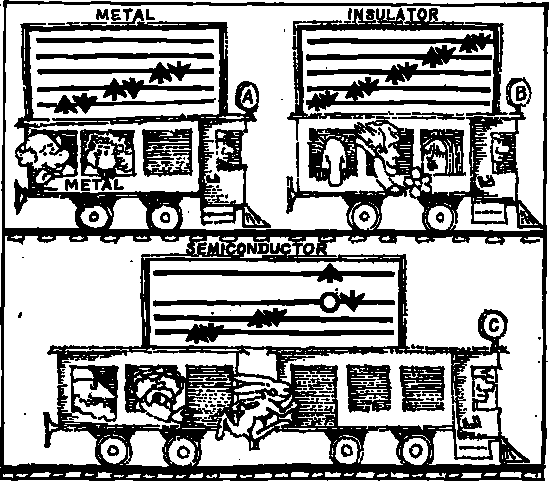
\includegraphics[width=\textwidth]{figures/fig-02-09.pdf}
\caption{Electrons bands in insulators, metals and semiconductors.}
\label{fig-2.9}
\end{figure}


This picture clearly explains the division of solids according to their electrical conductivity into metals, semiconductors and insulators (\figr{fig-2.9}). When a band is completely filled with electrons and the width of the gap to the next higher empty band is large, the body is an insulator, or nonconductor. If the upper band is only partly filled with electrons, we have a metal because even the weakest electric field can kick an electron to a slightly higher energy level. Typical of a semiconductor is the fact that its upper band is separated from the next lower one by a narrow gap. In contrast to nonconductors and metals, thermal motion is capable in semiconductors of transferring electrons from one band to another. In the absence of a field, the number of such transitions upward and downward are the same. A rise in temperature only increases the electron concentration in the upper band.

But what happens when a field is applied to semiconductor?

Now a free electron in the upper band begins to move and contributes to the negative conduction. But the equilibrium of upward and downward electron transitions is violated. Therefore a hole is formed in the lower band and begins to move, due to the field, in the opposite direction. Such semiconductors are called \emph{conductors with mixed (positive-negative) conduction}.


The band theory of semiconductors is an orderly and consistent one. The reader should not consider the described model to be artificial or far-fetched. It simply and clearly explains the principal difference between a metal and a semiconductor, namely, their particular behaviour with a change in temperature. As mentioned
in a preceding section, the electrical conductivity of metals drops with a rise in temperature because the electrons more frequently collide with obstacles. An increase in the temperature of a semiconductor leads to an increase in the number of electrons and holes, and a consequent increase in conductivity. Calculations indicate that this effect substantially exceeds the loss in conductivity due to collisions with obstacles.

Of prime importance in engineering are semiconductors with impurities. By adding impurities, called \emph{doping}, we can produce a body that has only negative or only positive conduction. The idea is extremely simple.

The most extensively employed semiconductor materials are germanium and silicon. These elements are tetravalent. Each atom is bound to four neighbours. Ideally pure germanium is a semiconductor of the mixed type. The number of holes and free electrons per \SI{1}{\centi\meter\cubed} is very small, namely, about \num{2.5d13}. This comes to about one free electron and one hole per thousand million atoms.


Now let us replace an atom of germanium with an atom of arsenic. Arsenic is pentavalent (having five valence electrons). Four of its electrons bind it to atoms of the host -- germanium -- and the fifth is free. This material possesses electron (negative) conduction because the addition of an arsenic atom does not lead to the formation of holes.

Even if only a trace of arsenic is added, one atom per million atoms of germanium, the conductivity of the germanium increases by a thousandfold.

It should be clear now what is needed to convert the germanium into a $p$-type conductor. This can be done by replacing a germanium atom with a trivalent atom, for example, indium.

This leads to the following situation. An atom of germanium adjacent to the guest is converted into a positive ion because it must form a bond with the indium, which has one electron too few. But we already know that a positive ion plays the role of a hole. Owing to the field, the holes move and there is motion of free electrons.

No wonder that the semiconductor industry has greatly influenced the techniques of growing pure crystals. It could not be otherwise when even a trace of impurities,
as small as a millionth part, makes all the difference. 

It would be incorrect to suppose that there is no hole conduction in $n$-type semiconductors. There are holes, of course, but their number is substantially less than the number of free electrons. In $n$-type semiconductors, the electrons are the \emph{majority carriers} of current, while the holes, constituting a minority, are called \emph{minority carriers}. On the contrary, the majority carriers in $p$-type semiconductors are holes, and the minority carriers are electrons.

\section{\emph{p-n} Junction}

Now that we know what $p$- and $n$-type semiconductors are, we can look into an interesting effect that is vitally important in up-to-date electronics. This effect occurs in the transition region between $p$- and $n$-type semiconductors tightly joined together. This region is commonly called a $p\!-\!n$ junction, though the word \emph{transition} has served as the basis for naming a whole class of devices (called transition-region devices) operating on the $p\!-\!n$ junction principle. What happens when we take two blocks of the same cross section, one made of \ce{Ge} doped with In ($p$-type semiconductor) and the other of \ce{Ge} doped with \ce{As}, grind one face on each block to an exceptionally high degree of smoothness and flatness! and join the ground faces very tightly together? We shall have, actually, a single crystal of germanium, but one half has an excess of free electrons and the other, an excess of holes.


To keep the explanation as simple as possible we shall, for the moment, forget about the minority current carriers. At the initial instant of time (see upper drawing in \figr{fig-2.10}), both halves of the crystal are electrically neutral. But the $n$-type half has (notwithstanding its electrical neutrality) ``surplus'' electrons (black dots) and the $p$-type half has ``surplus'' holes (circles).

Both the electrons and holes can freely pass through the boundary. The reason for such transitions is the same as in mixing two gases when their containers are connected together. But, in contrast to gas molecules, electrons and holes are capable of recombining.

\begin{figure}[!ht]
\centering
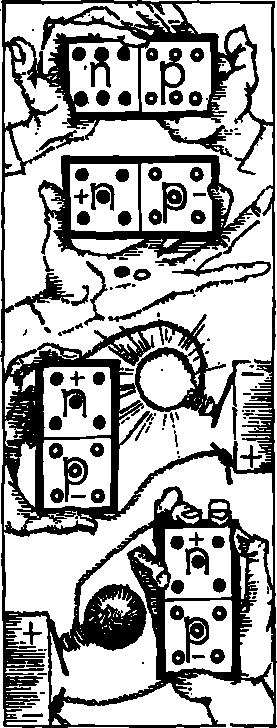
\includegraphics[width=0.4\textwidth]{figures/fig-02-10.pdf}
\caption{Conduction via a $p\!-\!n$ junction.}
\label{fig-2.10}
\end{figure}

At first we had six black dots at the left and six circles at the right. As soon as the transition begins, a circle and a dot annihilate each other. The next drawing shows that there are less electrons left in the left half than are required for it to remain electrically neutral. The right half has one circle less. Depleting the left half of one electron, we give this half a positive charge. For the same reason, the right half acquires a negative charge.

Transition through the boundary of the next holes and electrons becomes difficult. They have to move against the electric fields set up by the charges. Transition continues for some time, as long as the thermal motion is able to surmount the constantly increasing barrier. Finally, dynamic equilibrium is reached.

Now, what happens if we apply a voltage across our composite $p\!-\!n$ crystal as shown in the third drawing in \figr{fig-2.10}. Evidently, we submit additional energy to the current carriers of an amount sufficient to enable them to clear the barrier.

On the contrary, if we connect the positive pole to the $n$-type half, it remains impossible for electrons and holes to surmount the barrier.

In short, a $p\!-\!n$ junction allows current to flow in only one direction, thereby possessing rectifying properties. 

Today, rectifiers (for which valves and diodes are synonyms) find most extensive application in many different fields of engineering. Their principle has just been described.

Our explanation, however, was extremely crude. In no detail did it take into account the behaviour of the holes and electrons capable of surmounting the barrier without recombination. The main drawback was our disregard for the minority carriers that do not allow a $p\!-\!n$ crystal to completely rectify a current. Actually, a weak current does flow when we apply the voltage as shown in the lower drawing of \figr{fig-2.10}.

Let us consider in more detail the events that occur at the boundary, or junction, when dynamic equilibrium is reached.

We first discard the simple assumption we made above and recall the existence of minority carriers.

In establishing dynamic equilibrium, the situation is as follows. Approaching the boundary from the depth of the $p$-type crystal, the hole current gradually increases. Contributing to this current are holes that manage to reach the $p\!-\!n$ junction and jump across it without recombining with electrons.

Of course, these holes must also possess sufficient energy to overcome the potential barrier.

In passing through the transition region, this current gradually fades due to recombination with electrons. At the same time, a hole current gradually increases from the depth of the $n$-type crystal, flowing in the opposite direction. There are much fewer holes in this part, but they do not have to surmount the barrier to get into the $p$-type part. We can say that the barrier is arranged so that the forward and reverse currents compensate each other.

The above also concerns electron current. True, the hole and electron currents may differ greatly in magnitude because the $p$- and $n$-type parts are differently doped with impurities and possess, consequently, different amounts of free carriers. If, for instance, there are a great many more holes in the $p$-type part than electrons in the $n$-type part, the hole current is much higher than the electron current. Such a $p$-type part is called the \emph{emitter} of free current carriers, and the $n$-type part, the base.

After this more detailed account of the events happening at the $p\!-\!n$ boundary, we can understand why the current cannot be completely rectified.

As a matter of fact, if the positive pole is connected to the $p$-type crystal (or half), the barrier is lowered. The voltage drives the electrons ahead. If the positive pole is connected to the $n$-type part, the electric-field set up by the power source coincides in direction with that of the barrier. The field in the junction is increased. Now the number of electrons capable of surmounting the barrier, as well as the number of holes capable of moving in the opposite direction, are reduced. This raises the resistance in the junction region, leading to the so-called asymmetric volt-ampere characteristic.

As we can now see, a more thorough consideration clearly explains why the rectification in the junction layer cannot be complete.









